%-------------------------------------------------------
% SLEPc Users Manual
%-------------------------------------------------------
\chapter{\label{cap:st}ST: Spectral Transformation}
%-------------------------------------------------------

\noindent The Spectral Transformation (\ident{ST}) is the object that encapsulates the functionality required for acceleration techniques based on the transformation of the spectrum. Most eigensolvers in \ident{EPS} work by applying an operator to a set of vectors and this operator can adopt different forms. The \ident{ST} object handles all the different possibilities in a uniform way, so that the solver can proceed without knowing which transformation has been selected. The spectral transformation can be specified at run time, as well as related options such as which linear solver to use.

	Despite being a rather unrelated concept, \ident{ST} is also used to handle the preconditioners and correction-equation solvers used in preconditioned eigensolvers such as GD and JD.

	The description in this chapter focuses on the use of \ident{ST} in the context of \ident{EPS}. For usage within other solver classes, we will provide further details, e.g., shift-and-invert for polynomial eigenproblems in \S\ref{sec:qst}.

%---------------------------------------------------
\section{General Description}

	Spectral transformations are powerful tools for adjusting the way in which eigensolvers behave when coping with a problem. The general strategy consists in transforming the original problem into a new one in which eigenvalues are mapped to a new position while eigenvectors remain unchanged. These transformations can be used with several goals in mind:
\begin{itemize}
\setlength{\itemsep}{-2pt}
\item Compute internal eigenvalues. In some applications, the eigenpairs of interest are not the extreme ones (largest magnitude, smallest magnitude, rightmost, leftmost), but those contained in a certain interval or those closest to a certain value of the complex plane.
\item Accelerate convergence. Convergence properties typically depend on how close the eigenvalues are from each other. With some spectral transformations, difficult eigenvalue distributions can be remapped in a more favorable way in terms of convergence. 
\item Handle some special situations. For instance, in generalized problems when matrix $B$ is singular, it may be necessary to use a spectral transformation.
\end{itemize}
	
	\slepc separates spectral transformations from solution methods so that any combination of them can be specified by the user. To achieve this, most eigensolvers contained in \ident{EPS} are implemented in such a way that they are independent of which transformation has been selected by the user (the exception are preconditioned solvers, see below). That is, the solver algorithm has to work with a generic operator, whose actual form depends on the transformation used. After convergence, eigenvalues are transformed back appropriately. 

	For technical details of the transformations described in this chapter, the interested user is referred to \citep{Ericsson:1980:STL}, \citep{Scott:1982:AIO}, \citep{Nour-Omid:1987:HIS}, and \citep{Meerbergen:1994:SCT}.

\paragraph{Preconditioners.}

As explained in the previous chapter, \ident{EPS} contains preconditioned eigensolvers such as GD or JD. These solvers either apply a preconditioner at a certain step of the computation, or need to solve a correction equation with a preconditioned linear solver. One of the main goals of these solvers is to achieve a similar effect as an inverse-based spectral transformation such as shift-and-invert, but with less computational cost. For this reason, a ``preconditioner'' spectral transformation has been included in the \ident{ST} object. However, this is just a convenient way of organizing the functionality, since this fake spectral transform cannot be used with non-preconditioned eigensolvers, and conversely preconditioned eigensolvers cannot be used with conventional spectral transformations.

%---------------------------------------------------
\section{Basic Usage}

	The \ident{ST} module is the analog of some \petsc modules such as \texttt{PC}. The user does not usually need to create a stand-alone \ident{ST} object explicitly. Instead, every \ident{EPS} object internally sets up an associated \ident{ST}. Therefore, the usual object management methods such as \ident{STCreate}, \ident{STDestroy}, \ident{STView}, \ident{STSetFromOptions}, are not usually called by the user.

	Although the \ident{ST} context is hidden inside the \ident{EPS} object, the user still has control over all the options, by means of the command line, or also inside the program. To allow application programmers to set any of the spectral transformation options directly within the code, the following routine is provided to extract the \ident{ST} context from the \ident{EPS} object,
	\findex{EPSGetST}
	\begin{Verbatim}[fontsize=\small]
	EPSGetST(EPS eps,ST *st);
	\end{Verbatim}
	
	After this, one is able to set any options associated with the \ident{ST} object. For example, to set the value of the shift, the following function is available
	\findex{STSetShift}
	\begin{Verbatim}[fontsize=\small]
	STSetShift(ST st,PetscScalar shift);
	\end{Verbatim}
	This can also be done with the command line option \Verb!-st_shift <shift>!. Note that the argument \texttt{shift} is defined as a \texttt{PetscScalar}, and this means that complex shifts are not allowed unless the complex version of \slepc is used.

	Other object operations are available, which are not usually called by the user. The most important of such functions are \ident{STApply}, which applies the operator to a vector, and \ident{STSetUp}, which prepares all the necessary data structures before the solution process starts. The term ``operator'' refers to one of $A$, $B^{-1}\!A$, $A-\sigma I$, ...\ depending on which kind of spectral transformation is being used.
 
%---------------------------------------------------
\section{Available Transformations}

	This section describes the spectral transformations that are provided in \slepc. As in the case of eigensolvers, the spectral transformation to be used can be specified procedurally or via the command line. The application programmer can set it by means of the command
	\findex{STSetType}
	\begin{Verbatim}[fontsize=\small]
	STSetType(ST st,STType type);
	\end{Verbatim}
where \texttt{type} can be one of 
\texttt{STSHIFT}, 
\texttt{STSINVERT}, \texttt{STCAYLEY},
\texttt{STPRECOND}, or \texttt{STSHELL}.
The \ident{ST} type can also be set with the command-line option \Verb!-st_type! followed by the name of the method (see Table \ref{tab:transforms}). The first five spectral transformations are described in detail in the rest of this section. The last possibility, \texttt{STSHELL}, uses a specific, application-provided spectral transformation. Section \ref{sec:shell} describes how to implement one of these transformations.

\begin{table}
\centering
{\small \begin{tabular}{lllc}
                        &                   & {\footnotesize Options} &\\
Spectral Transformation & \ident{STType}    & {\footnotesize Name}    & Operator\\\hline
Shift of Origin         & \texttt{STSHIFT}  & \texttt{shift}   & $B^{-1}A-\sigma I$\\
Shift-and-invert        & \texttt{STSINVERT}& \texttt{sinvert} & $(A-\sigma B)^{-1}B$\\
Generalized Cayley      & \texttt{STCAYLEY} & \texttt{cayley}  & $(A-\sigma B)^{-1}(A+\nu B)$\\
Preconditioner          & \texttt{STPRECOND}& \texttt{precond} & $K^{-1}\approx(A-\sigma B)^{-1}$\\\hline
Shell Transformation    & \texttt{STSHELL}  & \texttt{shell}   & \emph{user-defined}\\\hline
\end{tabular} }
\caption{\label{tab:transforms}Spectral transformations available in the  \ident{ST} package.}
\end{table}

	The last column of Table \ref{tab:transforms} shows a general form of the operator used in each case. This generic operator can adopt different particular forms depending on whether the eigenproblem is standard or generalized, or whether the value of the shift ($\sigma$) and anti-shift ($\nu$) is zero or not. All the possible combinations are listed in Table \ref{tab:op}.
	\begin{table}
	\centering
	{\small \begin{tabular}{llcc}
	\ident{ST}     & Choice of $\sigma,\nu$ & Standard problem & Generalized problem \\\hline
	\texttt{shift}
        & $\sigma=0$     & $A$           & $B^{-1}A$          \\
	& $\sigma\not=0$ & $A-\sigma I$  & $B^{-1}A-\sigma I$ \\ \hline
	\texttt{sinvert}
        & $\sigma=0$     & $A^{-1}$      & $A^{-1}B$          \\
	& $\sigma\not=0$ & $(A-\sigma I)^{-1}$  & $(A-\sigma B)^{-1}B$ \\ \hline
	\texttt{cayley}
	& $\sigma\not=0,\nu=0$ & $(A-\sigma I)^{-1}A$  & $(A-\sigma B)^{-1}A$ \\
        & $\sigma=0,\nu\not=0$     & $I+\nu A^{-1}$      & $I+\nu A^{-1}B$ \\
	& $\sigma\not=0,\nu\not=0$ & $(A-\sigma I)^{-1}(A+\nu I)$  & $(A-\sigma B)^{-1}(A+\nu B)$ \\ \hline
	\texttt{precond}
        & $\sigma=0$     & $K^{-1}\approx A^{-1}$ & $K^{-1}\approx A^{-1}$          \\
	& $\sigma\not=0$ & $K^{-1}\approx(A-\sigma I)^{-1}$ & $K^{-1}\approx(A-\sigma B)^{-1}$ \\ \hline
	\end{tabular} }
	\caption{\label{tab:op}Operators used in each spectral transformation mode.}
	\end{table}

	The expressions shown in Table \ref{tab:op} are not built explicitly. Instead, the appropriate operations are carried out when applying the operator to a certain vector. The inverses imply the solution of a linear system of equations that is managed by setting up an associated \ident{KSP} object. The user can control the behavior of this object by adjusting the appropriate options, as will be illustrated with examples in \S\ref{sec:lin}.

\paragraph{Relation between Target and Shift.}

	In all transformations except \ident{STSHIFT}, there is a direct connection between the target $\tau$ (described in \S\ref{sec:defprob}) and the shift $\sigma$, as will be discussed below. The normal usage is that the user sets the target and then $\sigma$ is set to $\tau$ automatically (though it is still possible for the user to set a different value of the shift).

\subsection{Shift of Origin}

	By default, no spectral transformation is performed. This is equivalent to a shift of origin (\texttt{STSHIFT}) with $\sigma=0$, that is, the first line of Table \ref{tab:op}. The solver works with the original expressions of the eigenvalue problems,
\begin{equation}Ax=\lambda x,\end{equation}
for standard problems, and $Ax=\lambda Bx$ for generalized ones. Note that this last equation is actually treated internally as
\begin{equation}B^{-1}Ax=\lambda x.\end{equation}
When the eigensolver in \ident{EPS} requests the application of the operator to a vector, a matrix-vector multiplication by matrix $A$ is carried out (in the standard case) or a matrix-vector multiplication by matrix $A$ followed by a linear system solve with coefficient matrix $B$ (in the generalized case). Note that in the last case, the operation will fail if matrix $B$ is singular.

When the shift, $\sigma$, is given a value different from the default, 0, the effect is to move the whole spectrum by that exact quantity, $\sigma$, which is called \emph{shift of origin}. To achieve this, the solver works with the shifted matrix, that is, the expressions it has to cope with are
\begin{equation}(A-\sigma I)x=\theta x,\end{equation}
for standard problems, and 
\begin{equation}(B^{-1}A-\sigma I) x=\theta x,\end{equation}
for generalized ones. The important property that is used is that shifting does not alter the eigenvectors and that it does change the eigenvalues in a simple known way, it shifts them by $\sigma$. In both the standard and the generalized problems, the following relation holds 
\begin{equation}\theta=\lambda-\sigma.\end{equation}
This means that after the solution process, the value $\sigma$ has to be added\footnote{Note that the sign changed in \slepc 3.5 with respect to previous versions.} to the computed eigenvalues, $\theta$, in order to retrieve the solution of the original problem, $\lambda$. This is done by means of the function \ident{STBackTransform}, which does not need to be called directly by the user.

\subsection{Shift-and-invert}

  \begin{figure}[t]
    \centering
    \begin{tikzpicture}
      \draw[->] (-1.5,0) -- (5.5,0) node[right] {$\lambda$};
      \draw[->] (0,-4) -- (0,4) node[above] {$\theta$};
      \draw[dashed,color=gray] (2,-4) -- (2,4);
      %\draw[color=blue] plot[id=sinv1,domain=-1.3:1.75] function{1/(x-2)};
      \draw[color=blue] 
        (-1.30000,-0.30303) -- (-1.17292,-0.31517) -- (-1.04583,-0.32832) --
        (-0.91875,-0.34261) -- (-0.79167,-0.35821) -- (-0.66458,-0.37529) --
        (-0.53750,-0.39409) -- (-0.41042,-0.41487) -- (-0.28333,-0.43796) --
        (-0.15625,-0.46377) -- (-0.02917,-0.49281) -- ( 0.09792,-0.52574) --
        ( 0.22500,-0.56338) -- ( 0.35208,-0.60683) -- ( 0.47917,-0.65753) --
        ( 0.60625,-0.71749) -- ( 0.73333,-0.78947) -- ( 0.86042,-0.87751) --
        ( 0.98750,-0.98765) -- ( 1.11458,-1.12941) -- ( 1.24167,-1.31868) --
        ( 1.36875,-1.58416) -- ( 1.49583,-1.98347) -- ( 1.62292,-2.65193) --
        ( 1.75000,-4.00000);
      %\draw[color=blue] plot[id=sinv2,domain=2.25:5.3] function{1/(x-2)};
      \draw[color=blue] 
        (2.25000,4.00000) -- (2.37708,2.65193) -- (2.50417,1.98347) --
        (2.63125,1.58416) -- (2.75833,1.31868) -- (2.88542,1.12941) --
        (3.01250,0.98765) -- (3.13958,0.87751) -- (3.26667,0.78947) --
        (3.39375,0.71749) -- (3.52083,0.65753) -- (3.64792,0.60683) --
        (3.77500,0.56338) -- (3.90208,0.52574) -- (4.02917,0.49281) --
        (4.15625,0.46377) -- (4.28333,0.43796) -- (4.41042,0.41487) --
        (4.53750,0.39409) -- (4.66458,0.37529) -- (4.79167,0.35821) --
        (4.91875,0.34261) -- (5.04583,0.32832) -- (5.17292,0.31517) --
        (5.30000,0.30303);
      \node[below right] at (0,0) {$0$};
      \draw (2,0.1) -- (2,-0.1) node[below left] at (2,0) {$\sigma$};
      \node at (4,3.2) {$\theta = \frac{1}{\lambda-\sigma}$};
      \draw[very thin,color=gray] (2.5,0) |- (0,2);
      \draw[very thin,color=gray] (3.9,0) |- (0,0.5263);
      \foreach \pos/\label in {2/$\theta_1$,0.5263/$\theta_2$}
      \draw (-0.1,\pos) -- (0.1,\pos) (-0.8mm,\pos cm) node[anchor=east,font=\footnotesize] {\label};
      \foreach \pos/\label in {2.5/$\lambda_1$,3.9/$\lambda_2$}
      \draw (\pos,0.1) -- (\pos,-0.1) (\pos cm,-2.5ex) node[anchor=base,font=\footnotesize] {\label};
    \end{tikzpicture}
    \caption{\label{fig:sinvert}The shift-and-invert spectral transformation.}
  \end{figure}

	The shift-and-invert spectral transformation (\texttt{STSINVERT}) is used to enhance convergence of eigenvalues in the neighborhood of a given value. In this case, the solver deals with the expressions 
\begin{eqnarray}
(A-\sigma I)^{-1}x=\theta x,\\
(A-\sigma B)^{-1}B x=\theta x,
\end{eqnarray}
for standard and generalized problems, respectively. 
This transformation is effective for finding eigenvalues near $\sigma$ since the eigenvalues $\theta$ of the operator that are largest in magnitude correspond to the eigenvalues $\lambda$ of the original problem that are closest to the shift $\sigma$ in absolute value, as illustrated in Figure \ref{fig:sinvert} for an example with real eigenvalues. Once the wanted eigenvalues have been found, they may be transformed back to eigenvalues of the original problem. Again, the eigenvectors remain unchanged.
In this case, the relation between the eigenvalues of both problems is
\begin{equation}\theta=1/(\lambda-\sigma).\end{equation}
Therefore, after the solution process, the operation to be performed in function \ident{STBackTransform} is $\lambda=\sigma+1/\theta$ for each of the computed eigenvalues.

This spectral transformation is used in the spectrum slicing technique, see \S\ref{sec:slice}.

\subsection{Cayley}
\label{sec:cayley}

	The generalized Cayley transform (\texttt{STCAYLEY}) is defined from the expressions
\begin{eqnarray}
(A-\sigma I)^{-1}(A+\nu I)x=\theta x,\\
(A-\sigma B)^{-1}(A+\nu B)x=\theta x,
\end{eqnarray}
for standard and generalized problems, respectively. Sometimes, the term Cayley transform is applied for the particular case in which $\nu=\sigma$. This is the default if $\nu$ is not given a value explicitly. The value of $\nu$ (the anti-shift) can be set with the following function
	\findex{STCayleySetAntishift}
	\begin{Verbatim}[fontsize=\small]
	STCayleySetAntishift(ST st,PetscScalar nu);
	\end{Verbatim}
or in the command line with \Verb!-st_cayley_antishift!.

This transformation is mathematically equivalent to shift-and-invert and, therefore, it is effective for finding eigenvalues near $\sigma$ as well. However, in some situations it is numerically advantageous with respect to shift-and-invert (see \citep[\S 11.2]{Bai:2000:TSA}, \citep{Lehoucq:2001:LEC}).

In this case, the relation between the eigenvalues of both problems is
\begin{equation}\theta=(\lambda+\nu)/(\lambda-\sigma).\end{equation}
Therefore, after the solution process, the operation to be performed in function \ident{STBackTransform} is $\lambda=(\theta\sigma+\nu)/(\theta-1)$ for each of the computed eigenvalues.

\subsection{Preconditioner}
\label{sec:precond}

	As mentioned in the introduction of this chapter, the special type \ident{STPRECOND} is used for handling preconditioners or preconditioned iterative linear solvers, which are used in the context of preconditioned eigensolvers for expanding the subspace. For instance, in the GD solver the so-called correction vector $d_i$ to be added to the subspace in each iteration is computed as
\begin{equation}
d_i=K^{-1}P_i(A-\theta_i B)x_i,
\end{equation}
where $(\theta_i,x_i)$ is the current approximation of the sought-after eigenpair, and $P_i$ is a projector involving $x_i$ and $K^{-1}x_i$. In the above expressions, $K$ is a preconditioner matrix that is built from $A-\theta_i B$. However, since $\theta_i$ changes at each iteration, which would force recomputation of the preconditioner, we opt for using
\begin{equation}
\label{eq:precon}
K^{-1}\approx (A-\sigma B)^{-1}.
\end{equation}

	Similarly, in the JD eigensolver the expansion of the subspace is carried out by solving a correction equation similar to
\begin{equation}
(I-x_ix_i^*)(A-\theta_i B)(I-x_ix_i^*)d_i=-(A-\theta_i B)x_i,
\end{equation}
where the system is solved approximately with a preconditioned iterative linear solver. For building the preconditioner of this linear system, the projectors $I-x_ix_i^*$ are ignored, and again it is not recomputed in each iteration. Therefore, the preconditioner is built as in expression \ref{eq:precon} as well.

	It should be clear from the previous discussion, that \ident{STPRECOND} does not work in the same way as the rest of spectral transformations. In particular, it is not intended to be used on the basis of operator applications with \ident{STApply}, and it does not rely on \ident{STBackTransform} either. It is rather a convenient mechanism for handling the preconditioner and linear solver (see examples in \S\ref{sec:lin}). The expressions shown in Tables \ref{tab:transforms} and \ref{tab:op} are just a reference to indicate from which matrix the preconditioner is built by default.

	There is the possibility that the user overrides the default behaviour, that is, to explicitly supply a matrix from which the preconditioner is to be built, with
	\findex{STPrecondSetMatForPC}
	\begin{Verbatim}[fontsize=\small]
	STPrecondSetMatForPC(ST st,Mat mat);
	\end{Verbatim}

	Note that preconditioned eigensolvers in \ident{EPS} select \ident{STPRECOND} by default, so the user does not need to specify it explicitly.

%---------------------------------------------------
\section{Advanced Usage}

Using the \ident{ST} object is very straightforward. However, when using spectral transformations many things are happening behind the scenes, mainly the solution of linear systems of equations. The user must be aware of what is going on in each case, so that it is possible to guide the solution process in the most beneficial way. This section describes several advanced aspects that can have a considerable impact on efficiency.

\subsection{Solution of Linear Systems}
\label{sec:lin}

	In many of the cases shown in Table \ref{tab:op}, the operator contains an inverted matrix, which means that a linear system of equations must be solved whenever the application of the operator to a vector is required. These cases are handled internally by means of a \ident{KSP} object.

	In the simplest case, a generalized problem is to be solved with a zero shift. Suppose you run a program that solves a generalized eigenproblem, with default options:
\begin{Verbatim}[fontsize=\small]
	$ ./program
\end{Verbatim}
In this case, the \ident{ST} object associated with the \ident{EPS} solver creates a \ident{KSP} object whose coefficient matrix is $B$. By default, this \ident{KSP} object is set to use a direct solver\footnote{This is the default since \slepc 3.0.0.}, in particular an LU factorization. However, default settings can be changed, as illustrated below.

	The following command-line is equivalent to the previous one:
\begin{Verbatim}[fontsize=\small]
	$ ./program -st_ksp_type preonly -st_pc_type lu
\end{Verbatim}
The two options specify the type of the linear solver and preconditioner to be used. The \Verb!-st_! prefix indicates that the option corresponds to the linear solver within \ident{ST}. The combination \texttt{preonly}$+$\texttt{lu} instructs to use a direct solver (LU factorization, see \petsc's documentation for details), so this is the same as the default. Adding a new option changes the default behaviour, for instance
\begin{Verbatim}[fontsize=\small]
	$ ./program -st_ksp_type preonly -st_pc_type lu
                    -st_pc_factor_mat_solver_package mumps
\end{Verbatim}
In this case, an external linear solver package is used (MUMPS, see \petsc's documentation for other available packages). Note that an external package is required for computing a matrix factorization in parallel, since \petsc itself only provides sequential direct linear solvers.

	Instead of a direct linear solver, it is possible to use an iterative solver. This may be necessary in some cases, specially for very large problems. However, the user is warned that using an iterative linear solver makes the overall solution process less robust (see also the discussion of preconditioned eigensolvers below). As an example, the command-line
\begin{Verbatim}[fontsize=\small]
	$ ./program -st_ksp_type gmres -st_pc_type bjacobi -st_ksp_rtol 1e-9
\end{Verbatim}
selects the GMRES solver with block Jacobi preconditioning. In the case of iterative solvers, it is important to use an appropriate tolerance, usually slightly more stringent for the linear solves relative to the desired accuracy of the eigenvalue calculation ($10^{-9}$ in the example, compared to $10^{-8}$ for the eigensolver). 

	Although the direct solver approach may seem too costly, note that the factorization is only carried out at the beginning of the eigenvalue calculation and this cost is amortized in each subsequent application of the operator. This is also the case for iterative methods with preconditioners with high-cost set-up such as ILU.

	The application programmer is able to set the desired linear systems solver options also from within the code. In order to do this, first the context of the \ident{KSP} object must be retrieved with the following function
	\findex{STGetKSP}
	\begin{Verbatim}[fontsize=\small]
	STGetKSP(ST st,KSP *ksp);
	\end{Verbatim}
	
	The above functionality is also applicable to the other spectral transformations. For instance, for the shift-and-invert technique with $\tau=10$ using BiCGStab+Jacobi:
\begin{Verbatim}[fontsize=\small]
	$ ./program -st_type sinvert -eps_target 10 -st_ksp_type bcgs -st_pc_type jacobi
\end{Verbatim}
	In shift-and-invert and Cayley, unless $\sigma=0$, the coefficient matrix is not a simple matrix but an expression that can be explicitly constructed or not, depending on the user's choice. This issue is examined in detail in \S\ref{sec:explicit} below.

In many cases, especially if a shift-and-invert or Cayley transformation is being used, iterative methods may not be well suited for solving linear systems (because of the properties of the coefficient matrix that can be indefinite and ill-conditioned). When using an iterative linear solver, it may be helpful to run with the option \Verb!-st_ksp_converged_reason!, which will display the number of iterations required in each operator application.
In extreme cases, the iterative solver fails, so \ident{EPSSolve} aborts with an error
\begin{Verbatim}[fontsize=\small]
	[0]PETSC ERROR: KSP did not converge (reason=DIVERGED_ITS)!
\end{Verbatim}
If this happens, it is necessary to use a direct method for solving the linear systems, as explained above.

\paragraph{The Case of Preconditioned Eigensolvers.}

	The \texttt{KSP} object contained internally in \ident{ST} is also used for applying the preconditioner or solving the correction equation in preconditioned eigensolvers.

	The GD eigensolver employs just a preconditioner. Therefore, by default it sets the \texttt{KSP} type to \texttt{preonly} (no other \texttt{KSP} is allowed) and the \texttt{PC} type to \texttt{jacobi}. The user may change the preconditioner, for example as
\begin{Verbatim}[fontsize=\small]
	$ ./ex5 -eps_type gd -st_pc_type asm
\end{Verbatim}

	The JD eigensolver uses both an iterative linear solver and a preconditioner, so both \texttt{KSP} and \texttt{PC} are meaningful in this case. The default is \texttt{gmres}+\texttt{bjacobi}. It is important to note that, contrary to the ordinary spectral transformations where a direct linear solver is recommended, in JD using an iterative linear solver is usually better than a direct solver. Indeed, the best performance may be achieved with a few iterations of the linear solver (or a large tolerance). For instance, the next example uses JD with GMRES+Jacobi limiting to 10 the number of allowed iterations for the linear solver:
\begin{Verbatim}[fontsize=\small]
	$ ./ex5 -eps_type jd -st_ksp_type gmres -st_pc_type jacobi -st_ksp_max_it 10
\end{Verbatim}

\subsection{Explicit Computation of Coefficient Matrix}
\label{sec:explicit}

	Three possibilities can be distinguished regarding the form of the coefficient matrix of the linear systems of equations associated with the different spectral transformations. The possible coefficient matrices are:
	\begin{itemize}
	\item Simple: $B$.
	\item Shifted: $A-\sigma I$.
	\item Axpy: $A-\sigma B$.
	\end{itemize}
	The first case has already been described and presents no difficulty. In the other two cases, there are three possible approaches:
	\begin{description}
	\item[``\Verb!shell!''] To work with the corresponding expression without forming the matrix explicitly. This is achieved by internally setting a matrix-free matrix with \ident{MatCreateShell}.
	\item[``\Verb!inplace!''] To build the coefficient matrix explicitly. This is done by means of a \ident{MatShift} or a \ident{MatAXPY} operation, which overwrites matrix $A$ with the corresponding expression. This alteration of matrix $A$ is reversed after the eigensolution process has finished.
	\item[``\Verb!copy!''] To build the matrix explicitly, as in the previous option, but using a working copy of the matrix, that is, without modifying the original matrix $A$. 
	\end{description}
	The default behavior is to build the coefficient matrix explicitly in a copy of $A$ (option ``\Verb!copy!''). The user can change this as in the following example
\begin{Verbatim}[fontsize=\small]
	$ ./program -st_type sinvert -eps_target 10 -st_ksp_type cg
                    -st_pc_type jacobi -st_matmode shell
\end{Verbatim}
	As always, the procedural equivalent is also available for specifying this option in the code of the program:
	\findex{STSetMatMode}
	\begin{Verbatim}[fontsize=\small]
	STSetMatMode(ST st,STMatMode mode);
	\end{Verbatim}

	The user must consider which approach is the most appropriate for the particular application. The different options have advantages and drawbacks. The first approach is the simplest one but severely restricts the number of possibilities available for solving the system, in particular most of the \petsc{} preconditioners would not be available, including direct methods. The only preconditioners that can be used in this case are Jacobi (only if matrices $A$ and $B$ have the operation \ident{MATOP\_GET\_DIAGONAL}) or a user-defined one.
	
	The second approach (``\Verb!inplace!'') can be much faster, specially in the generalized case. A more important advantage of this approach is that, in this case, the linear system solver can be combined with any of the preconditioners available in \petsc, including those which need to access internal matrix data-structures such as ILU. The main drawback is that, in the generalized problem, this approach probably makes sense only in the case that $A$ and $B$ have the same sparse pattern, because otherwise the function \ident{MatAXPY} might be inefficient. 
If the user knows that the pattern is the same (or a subset), then this can be specified with the function
	\findex{STSetMatStructure}
	\begin{Verbatim}[fontsize=\small]
	STSetMatStructure(ST st,MatStructure str);
	\end{Verbatim}
	
	Note that when the value of the shift $\sigma$ is very close to an eigenvalue, then the linear system will be ill-conditioned and using iterative methods may be problematic. On the other hand, in symmetric definite problems, the coefficient matrix will be indefinite whenever $\sigma$ is a point in the interior of the spectrum and in that case it is not possible to use a symmetric definite factorization (Cholesky or ICC).

	The third approach (``\Verb!copy!'') uses more memory but avoids a potential problem that could appear in the ``\Verb!inplace!'' approach: the recovered matrix might be slightly different from the original one (due to roundoff).

\subsection{Preserving the Symmetry in Generalized Eigenproblems}
\label{sec:symm}

	As mentioned in \S\ref{sec:defprob}, some eigensolvers can exploit symmetry and compute a solution for Hermitian problems with less storage and/or computational cost than other methods. Also, symmetric solvers can be more accurate in some cases. However, in the case of generalized eigenvalue problems in which both $A$ and $B$ are symmetric, it happens that, due to the spectral transformation, symmetry is lost since none of the transformed operators $B^{-1}\!A-\sigma I$, $(A-\sigma B)^{-1}B$, etc.\ is symmetric (the same applies in the Hermitian case for complex matrices).

	The solution proposed in \slepc is based on selecting different kinds of inner products. Currently, we have the following choice of inner products:
  \begin{itemize}
    \item Standard Hermitian inner product: $\langle x,y\rangle=x^*y$.
    \item $B$-inner product: $\langle x,y\rangle_B=x^*\!B\,y$.
  \end{itemize}

	The second one can be used for preserving the symmetry in symmetric definite generalized problems, as described below. Note that $\langle x,y\rangle_B$ is a genuine inner product only if $B$ is symmetric positive definite (for the case of symmetric positive semi-definite $B$ see \S\ref{sec:purif}). 

	It can be shown that $\mathbb{R}^n$ with the $\langle x,y\rangle_B$ inner product is isomorphic to the Euclidean $n$-space $\mathbb{R}^n$ with the standard Hermitian inner product. This means that if we use $\langle x,y\rangle_B$ instead of the standard inner product, we are just changing the way lengths and angles are measured, but otherwise all the algebraic properties are maintained and therefore algorithms remain correct. What is interesting to observe is that the transformed operators such as $B^{-1}\!A$ or $(A-\sigma B)^{-1}B$ are self-adjoint with respect to $\langle x,y\rangle_B$.

\begin{figure}
\centering
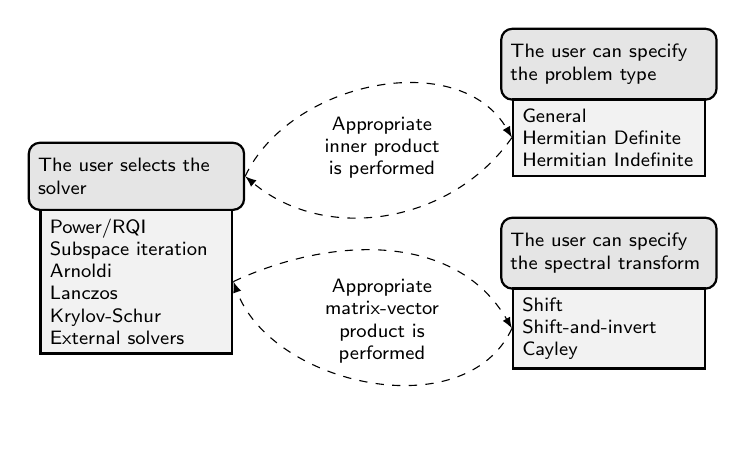
\begin{tikzpicture}
  \begin{scope}[every node/.style={draw,thick,text ragged,font=\sffamily\scriptsize},every to/.style={draw,-stealth,very thick,dashed}]
  \node[above right,rounded corners,fill=black!10,text width=2.5cm,inner ysep=2mm] (n1c) at (0,0)
       {The user selects the solver};
  \node[below right,fill=black!5,text width=2.2cm] (n1) at (0.15,0.03)
       {\begin{minipage}{\textwidth}Power/RQI\\Subspace iteration\\Arnoldi\\Lanczos\\
       Krylov-Schur\\External solvers\end{minipage}};
  \node[above right,rounded corners,fill=black!10,text width=2.5cm,inner ysep=2mm] (n2c) at (6,1.4)
       {The user can specify the problem type};
  \node[below right,fill=black!5,text width=2.2cm] (n2) at (6.15,1.43)
       {\begin{minipage}{\textwidth}General\\Hermitian Definite\\Hermitian Indefinite
       \end{minipage}};
  \node[above right,rounded corners,fill=black!10,text width=2.5cm,inner ysep=2mm] (n3c) at (6,-1.0)
       {The user can specify the spectral transform};
  \node[below right,fill=black!5,text width=2.2cm] (n3) at (6.15,-0.97)
       {\begin{minipage}{\textwidth}Shift\\Shift-and-invert\\Cayley
       \end{minipage}};
  \draw[dashed,-latex] (n1c.east) to[out=65,in=120] (n2.west);
  \draw[dashed,-latex] (n2.west) to[out=-125,in=-40] (n1c.east);
  \draw[dashed,-latex] (n1.east) to[out=25,in=120] (n3.west);
  \draw[dashed,-latex] (n3.west) to[out=-115,in=-70] (n1.east);
  \end{scope}
  \begin{scope}[every node/.style={text centered,text width=2cm,font=\sffamily\scriptsize}]
  \node at (4.5,.8) {Appropriate inner product is performed};
  \node at (4.5,-1.4) {Appropriate matrix-vector product is performed};
  \end{scope}
\end{tikzpicture}
\caption{\label{fig:abstr}Abstraction used by \slepc solvers.}
\end{figure}

	Internally, \slepc operates with the abstraction illustrated in Figure \ref{fig:abstr}. The operations indicated by dashed arrows are implemented as virtual functions. From the user point of view, all the above explanation is transparent. The only thing he/she has to care about is to set the problem type appropriately with \ident{EPSSetProblemType} (see \S\ref{sec:defprob}).
	In the case of the Cayley transform, \slepc is using $\langle x,y\rangle_{A+\nu B}$ as the inner product for preserving symmetry.

	Using the $B$-inner product may be attractive also in the non-symmetric case ($A$ non-symmetric) as described in the next subsection.

	Note that the above discussion is not directly applicable to \ident{STPRECOND} and the preconditioned eigensolvers, in the sense that the goal is not to recover the symmetry of the operator. Still, the $B$-inner product is also used in generalized symmetric-definite problems.

\subsection{Purification of Eigenvectors}
\label{sec:purif}

In generalized eigenproblems, the case of singular $B$ deserves especial consideration. In this case the default spectral transformation (\texttt{STSHIFT}) cannot be used since $B^{-1}$ does not exist.

In shift-and-invert with operator matrix $T=(A-\sigma B)^{-1}B$, when $B$ is singular all the eigenvectors that belong to finite eigenvalues are also eigenvectors of $T$ and belong to the range of $T$, $\mathcal{R}(T)$. In this case, the bilinear form $\langle x,y\rangle_B$ introduced in \S\ref{sec:symm} is a semi-inner product and $\|x\|_B=\sqrt{\langle x,x\rangle_B}$ is a semi-norm. As before, $T$ is self-adjoint with respect to this inner product since $B\,T=T^*B$. Also, $\langle x,y\rangle_B$ is a true inner product on $\mathcal{R}(T)$.

The implication of all this is that, for singular $B$, if the $B$-inner product is used throughout the eigensolver then, assuming that the initial vector has been forced to lie in $\mathcal{R}(T)$, the computed eigenvectors should be correct, i.e., they should belong to $\mathcal{R}(T)$ as well. Nevertheless, finite precision arithmetic spoils this nice picture, and computed eigenvectors are easily corrupted by components of vectors in the null-space of $B$. Additional computation is required for achieving the desired property. This is usually referred to as \emph{eigenvector purification}.

Although more elaborate purification strategies have been proposed (usually trying to reduce the computational effort, see \citep{Nour-Omid:1987:HIS} and \citep{Meerbergen:1997:IRA}), the approach in \slepc is simply to explicitly force the initial vector in the range of $T$, with $v_0\leftarrow Tv_0$, as well as the computed eigenvectors at the end, $x_i\leftarrow Tx_i$. Since this computation can be costly, it can be deactivated if the user knows that $B$ is non-singular, with
	\findex{EPSSetPurify}
	\begin{Verbatim}[fontsize=\small]
	EPSSetPurify(EPS eps,PetscBool purify);
	\end{Verbatim}

A final comment is that eigenvector corruption happens also in the non-symmetric case. If $A$ is non-symmetric but $B$ is symmetric positive semi-definite, then the scheme presented above ($B$-inner product together with purification) can still be applied and is generally more successful than the straightforward approach with the standard inner product. For using this scheme in \slepc, the user has to specify the special problem type \ident{EPS\_PGNHEP}, see Table \ref{tab:ptype}.

\subsection{Spectrum Slicing}
\label{sec:slice}

In the context of symmetric-definite generalized eigenvalue problems (\ident{EPS\_GHEP}) it is often required to compute all eigenvalues contained in a given interval $[a,b]$. This poses some difficulties, such as:
\begin{itemize}
\setlength{\itemsep}{0pt}
\item The number of eigenvalues in the interval is not known a priori.
\item There might be many eigenvalues, in some applications a significant percentage of the spectrum (20\%, say).
\item We must make certain that no eigenvalues are missed, and in particular all eigenvalues must be computed with their correct multiplicity.
\item In some applications, the interval is open in one end, i.e., either $a$ or $b$ can be infinite.
\end{itemize}
One possible strategy to solve this problem is to sweep the interval from one end to the other, computing chunks of eigenvalues with a spectral transformation that updates the shift dynamically. This is generally referred to as \emph{spectrum slicing}. The method implemented in \slepc is similar to that proposed by \cite{Grimes:1994:SBL}, where inertia information is used to validate sub-intervals. Given a symmetric-indefinite triangular factorization
\begin{equation}
A-\sigma B=LDL^T,
\end{equation}
by Sylvester's law of inertia we know that the number of eigenvalues on the left of $\sigma$ is equal to the number of negative eigenvalues of $D$,
\begin{equation}
\nu(A-\sigma B)=\nu(D).
\end{equation}
A detailed description of the method available in \slepc can be found in \citep{Campos:2012:SSS}.
The \slepc interface hides all the complications of the algorithm. However, the user must be aware of all the restrictions for this technique to be employed:
\begin{itemize}
\setlength{\itemsep}{0pt}
\item This is currently implemented only in Krylov-Schur.
\item The method is based on shift-and-invert, so \ident{STSINVERT} must be used. Furthermore, direct linear solvers are required.
\item The direct linear solver must provide the matrix inertia (see \petsc's \ident{MatGetInertia}). In particular, a symmetric factorization must be used (\texttt{cholesky}).
\end{itemize}

An example command-line that sets up all the required options is:
\begin{Verbatim}[fontsize=\small]
	$ ./ex12 -eps_interval 0.4,0.8 -st_type sinvert
                 -st_ksp_type preonly -st_pc_type cholesky
\end{Verbatim}

Note that \petsc's Cholesky factorization is not parallel, so for doing spectrum slicing in parallel it is required to use an external solver that supports inertia, e.g., MUMPS (see \S\ref{sec:lin} on how to use external linear solvers):
\begin{Verbatim}[fontsize=\small]
	$ ./ex12 -eps_interval 0.4,0.8 -st_type sinvert
                 -st_ksp_type preonly -st_pc_type cholesky
                 -st_pc_factor_mat_solver_package mumps -mat_mumps_icntl_13 1
\end{Verbatim}
The last option is required by MUMPS to compute the inertia.

Apart from the above recommendations, the following must be taken into account:
\begin{itemize}
\setlength{\itemsep}{0pt}
\item The parameters \texttt{nev} and \texttt{ncv} from \ident{EPSSetDimensions} are determined internally (user-provided values are ignored, and set to the number of eigenvalues in the interval). It is possible for the user to specify the ``local'' \texttt{nev} and \texttt{ncv} parameters that will be used when computing eigenvalues around each shift, with \ident{EPSKrylovSchurSetDimensions}.
\item The user can also tune the computation by setting different values of \texttt{max\_it}.
\end{itemize}

\paragraph{Use of multiple communicators}
Since spectrum slicing requires direct linear solves, parallel runs may suffer from bad scalability in the sense that increasing the number of MPI processes does not imply a performance gain. For this reason, \slepc provides the option of using multiple communicators, that is, splitting the initial MPI communicator in several groups, each of them in charge of processing part of the interval.

The multi-communicator setting is activated with a value of \texttt{npart}>1 in
	\findex{EPSKrylovSchurSetPartitions}
	\begin{Verbatim}[fontsize=\small]
	EPSKrylovSchurSetPartitions(EPS eps,PetscInt npart);
	\end{Verbatim}
The interval $[a,b]$ is then divided in \texttt{npart} subintervals of equal size, and the problem of computing all eigenvalues in $[a,b]$ is divided in \texttt{npart} independent subproblems. Each subproblem is solved using only a subset of the initial $p$ processes, with $\lceil p/\texttt{npart}\rceil$ processes at most. A final step will gather all computed solutions so that they are available in the whole \ident{EPS} communicator.

The division of the interval in subintervals is done blindly, and this may result in load imbalance if some subintervals contain much more eigenvalues than others. This can be prevented by passing a list of subinterval boundaries, provided that the user has a priori information to roughly determine the eigenvalue distribution:
	\findex{EPSKrylovSchurSetSubintervals}
	\begin{Verbatim}[fontsize=\small]
	EPSKrylovSchurSetSubintervals(EPS eps,PetscReal *subint);
	\end{Verbatim}

An additional benefit of multi-communicator support is that it enables parallel spectrum slicing runs without the need to install a parallel direct solver (MUMPS). The following command-line example uses sequential linear solves in 4 partitions, one process each:
\begin{Verbatim}[fontsize=\small]
	$ mpiexec -n 4 ./ex25 -eps_interval 0.4,0.8 -eps_krylovschur_partitions 4
                  -st_type sinvert -st_ksp_type preonly -st_pc_type cholesky
\end{Verbatim}

The analogue example using MUMPS with 5 processes in each partition:
\begin{Verbatim}[fontsize=\small]
	$ mpiexec -n 20 ./ex25 -eps_interval 0.4,0.8 -eps_krylovschur_partitions 4
                  -st_type sinvert -st_ksp_type preonly -st_pc_type cholesky
                  -st_pc_factor_mat_solver_package mumps -mat_mumps_icntl_13 1
\end{Verbatim}

\subsection{Spectrum Folding}

In \slepc versions prior to 3.5, \texttt{ST} had another type intended to perform the spectrum folding technique described below. It it no longer available with \texttt{ST}, but it can be implemented directly in application code as illustrated in example \texttt{ex24.c}.

Spectrum folding involves squaring in addition to shifting. This makes sense for standard Hermitian eigenvalue problems, where the transformed problem to be addressed is
\begin{equation}(A-\sigma I)^2x=\theta x.\end{equation}
The following relation holds 
\begin{equation}\theta=(\lambda-\sigma)^2.\end{equation}
Note that the mapping between $\lambda$ and $\theta$ is not injective, and hence this cannot be considered a true spectral transformation.

The effect is that the spectrum is folded around the value of $\sigma$. Thus, eigenvalues that are closest to the shift become the smallest eigenvalues in the folded spectrum, as illustrated in Figure \ref{fig:fold}. For this reason, spectrum folding is commonly used in combination with eigensolvers that compute the smallest eigenvalues, for instance in the context of electronic structure calculations, \citep{Canning:2000:PEP}. This transformation can be an effective, low-cost alternative to shift-and-invert.

  \begin{figure}
    \centering
    \begin{tikzpicture}[domain=-2:2]
      \draw[->] (-2.5,0) -- (2.5,0) node[right] {$\lambda$};
      \draw[->] (0,0) node[below] {$\sigma$} -- (0,4.2) node[above] {$\theta$};
      \draw[color=blue] 
          %plot[id=fold] function{x*x} 
          (-2.00000,4.00000) -- (-1.83333,3.36111) -- (-1.66667,2.77778) --
          (-1.50000,2.25000) -- (-1.33333,1.77778) -- (-1.16667,1.36111) --
          (-1.00000,1.00000) -- (-0.83333,0.69444) -- (-0.66667,0.44444) --
          (-0.50000,0.25000) -- (-0.33333,0.11111) -- (-0.16667,0.02778) --
          ( 0.00000,0.00000) -- ( 0.16667,0.02778) -- ( 0.33333,0.11111) --
          ( 0.50000,0.25000) -- ( 0.66667,0.44444) -- ( 0.83333,0.69444) --
          ( 1.00000,1.00000) -- ( 1.16667,1.36111) -- ( 1.33333,1.77778) --
          ( 1.50000,2.25000) -- ( 1.66667,2.77778) -- ( 1.83333,3.36111) --
          ( 2.00000,4.00000)
          node[right] {$\theta = (\lambda-\sigma)^2$};
      \draw[very thin,color=gray] (-1.3,0) |- (0,1.69);
      \draw[very thin,color=gray] (-0.5,0) |- (0,0.25);
      \draw[very thin,color=gray] (1.1,0) |- (0,1.21);
      \foreach \pos/\label in {1.69/$\theta_1$,0.25/$\theta_2$,1.21/$\theta_3$}
      \draw (-0.1,\pos) -- (0.1,\pos) (1mm,\pos cm) node[anchor=west,font=\footnotesize] {\label};
      \foreach \pos/\label in {-1.3/$\lambda_1$,-0.5/$\lambda_2$,1.1/$\lambda_3$}
      \draw (\pos,0.1) -- (\pos,-0.1) (\pos cm,-2.5ex) node[anchor=base,font=\footnotesize] {\label};
    \end{tikzpicture}
    \caption{\label{fig:fold}Illustration of the effect of spectrum folding.}
  \end{figure}


